% THIS IS AN EXAMPLE DOCUMENT FOR VLDB 2012
% based on ACM SIGPROC-SP.TEX VERSION 2.7
% Modified by  Gerald Weber <gerald@cs.auckland.ac.nz>
% Removed the requirement to include *bbl file in here. (AhmetSacan, Sep2012)
% Fixed the equation on page 3 to prevent line overflow. (AhmetSacan, Sep2012)

\documentclass{vldb}
\usepackage{times}
\usepackage{graphicx}
\usepackage{balance}  % for  \balance command ON LASMAD PAGE  (only there!)
\usepackage{alltt,algo}
\usepackage{url}
\usepackage{ctable} % Nicer tables, e.g., \toprule
\usepackage{verbatim} % Also provides the comment environment
\usepackage{dcolumn} % Decimal point alignment in tables
\usepackage{color} % for color comments

\makeatletter
% The vldb style file is an anachronsism. So no need to worry about hacks anyway.
% We redefined the listing environment by package minted here. (If we did not,
% we would also get an error because \aboveparskip is undefined.)
% Copied from vldb.csl
\@ifundefined{code}{\newcounter {code}} % this is for LaTeX2e

\def\fps@code{tbp}
\def\ftype@code{1}
\def\ext@code{lof}
\def\fnum@code{Listing \thecode}
\def\code{\@float{code}}
\let\endcode\end@float
\@namedef{code*}{\@dblfloat{code}}
\@namedef{endcode*}{\end@dblfloat}
\makeatother

\usepackage{minted}

% BEGIN Layout
	\newcommand{\otoprule}{\midrule[\heavyrulewidth]}
	
	\newcolumntype{+}{>{\global\let\currentrowstyle\relax}}
	\newcolumntype{^}{>{\currentrowstyle}}
	\newcommand{\rowstyle}[1]{\gdef\currentrowstyle{#1}%
		#1\ignorespaces
	}
% END Layout

% BEGIN Convenience commands
	% BEGIN Listing environments
	\newminted{cpp}{mathescape,
					linenos,
					numbersep=5pt,
					fontsize=\scriptsize,
					framesep=2mm}
	\newminted{python}{mathescape,
					  linenos,
					  numbersep=5pt,
					  fontsize=\scriptsize,
					  framesep=2mm}
	\newminted{sql}{mathescape,
					numbersep=5pt,
					tabsize=4,
					gobble=2,
					fontsize=\scriptsize,
					framesep=2mm}
	\newminted{psql}{numbersep=5pt,
					tabsize=4,
					gobble=2,
					fontsize=\scriptsize,
					framesep=2mm}
	% END Listing environments
	% BEGIN COMMENTS
  \newcommand{\jmh}[1]{{\textcolor{red}{#1 -- jmh}}}
  \newcommand{\fs}[1]{{\textcolor{orange}{#1 -- fs}}}
  % END COMMENTS
% END Convenience commands

% BEGIN Mathematical Definitions
	% BEGIN Set Symbols
		\newcommand{\setsymbol}[1]{\mathbb{#1}}
		\newcommand{\N}{\@ifstar{\setsymbol{N}_0}{\setsymbol{N}}}
		\newcommand{\R}{\setsymbol{R}}
	% END Set Symbols
	\renewcommand{\vec}[1]{\ensuremath{\boldsymbol{#1}}}
% END Mathematical Definitions



\begin{document}

% ****************** TITLE ****************************************

\title{Introducing MADlib\\{\Large (MAD Skills, the SQL)}}


\numberofauthors{11} %  in this sample file, there are a *total*
% of EIGHT authors. SIX appear on the 'first-page' (for formatting
% reasons) and the remaining two appear in the \additionalauthors section.

\author{Joseph M. Hellerstein\\{\small U.C. Berkeley} \and
 Christoper Re\\{\small U. Wisconsin} \and
 Florian Schoppmann\\{\small Greenplum} \and
 Daisy Zhe Wang\\{\small U. Florida} 
 % \and
 % Gavin Sherry\\{\small Greenplum} \and
 % Caleb Welton\\{\small Greenplum}
 % Eugene Fratkin\\{\small Greenplum} \and
 % Aleks Gorajek\\{\small Greenplum} \and
 % Steven Hillion\\{\small Alpine Data Labs} \and
 % Luke Lonergan\\{\small Greenplum} \and
 % Kee Siong Ng\\{\small Greenplum} \and 
 }

\maketitle

\begin{abstract}
  MADlib is a free, open-source library of in-database analytic methods.
  It provides an evolving suite of SQL-based algorithms for machine
  learning, data mining and statistics that run at scale within a
  database engine, with no need for data import/export to other tools.
  The goal is for MADlib to eventually serve a role for scalable
  database systems that is similar to the CRAN library for R: a
  community repository of statistical methods, this time written with
  scale and parallelism in mind.

  In this paper we introduce the MADlib project, including the
  background that led to its beginnings, and the motivation for its
  open-source nature.  We provide an overview of the library's
  architecture and design patterns, and provide a description
  of various statistical methods in that context.  We include raw performance and speedup results of a core design pattern from one of those methods over the Greenplum parallel DBMS on a modest-sized test cluster.    We then report on two 
  initial efforts at incorporating academic research into MADlib, which is one of the 
  project's goals. 
  
  MADlib is freely
  available in beta form at http://madlib.net, and the project is open
  for contributions of both new methods, and ports to additional
  database platforms.  
\end{abstract}




\section{Introduction:\\From Warehousing to Science}
\noindent
Until fairly recently, large databases were used mainly for accounting
purposes in enterprises, supporting financial record-keeping,
reporting and analysis at various levels of granularity.  {\em Data
Warehousing} was the name given to industry practices for these
database workloads.  Accounting, by definition, involves significant
care and attention to detail. Data Warehousing practices followed suit
by encouraging careful and comprehensive database design, and by following exacting policies regarding the quality of data loaded into the database.

Attitudes toward large databases have been changing quickly in the
past decade, as the focus of large database usage has shifted from
accountancy to analytics.  The need for correct accounting and data
warehousing practice has not gone away, but it is a becoming a
shrinking fraction of the volume---and the value---of large-scale data
management.  The emerging trend focuses on the use of a wide range of
potentially noisy data to support predictive analytics, managed by
statistical models and algorithms for analysis.  {\em Data Science} is a
name that is gaining currency for the industry practices evolving
around these workloads.

Data scientists make use of database engines in a very different way than traditional data warehousing professionals.  Rather than carefully
designing global schemas and ``repelling'' data until it is integrated,
they load data into private schemas in whatever form is convenient.  Rather than focusing on simple OLAP-style drill-down reports, they implement rich statistical
models and algorithms in the database, using extensible SQL as a
language for orchestrating data movement between disk, memory, and multiple parallel machines.  In short, for data scientists a DBMS is a scalable analytics runtime---one that is conveniently compatible with the database systems widely used for transactions and accounting.

In 2008, a group of us from the database industry, consultancy,
academia, and end-user analytics got together to describe this usage
pattern as we observed it in the field.  We dubbed it {\bf MAD}, an acronym for the {\em Magnetic} (as opposed to
repellent) aspect of the platform, the {\em Agile} design patterns used for
modeling, loading and iterating on data, and the {\em Deep} statistical models and
algorithms being used.  The ``MAD Skills'' paper that resulted described
this pattern, and included a number of non-trivial analytics
techniques implemented as simple SQL scripts~\cite{madskills}.

After the publication of the paper, it became clear that there was
significant interest not only in its design aspects, but
also in the actual SQL implementations of statistical methods.  This
interest came from every constituency involved: customers were
requesting it of consultants and vendors, and academics were
increasingly publishing papers on the topic.  What was missing was a
software framework to focus the energy of the community, and connect
the various interested constituencies.  This led to the design of
{\bf MADlib}, the subject of this paper.  

\subsection*{Introducing MADlib}
MADlib is a library of analytic methods that can be installed and
executed within a relational database engine that supports extensible
SQL.  A snapshot of the current contents of MADlib including methods and
ports is provided in Table~\ref{tab:methods} and Table~\ref{tab:ports}.  This set of methods and ports is intended to grow over time.

The methods in MADlib are designed for the shared-nothing, ``scale-out''
parallelism offered by modern parallel database engines, ensuring that
computation is done close to the data.  The core functionality is
written in declarative SQL statements, which orchestrate massively
parallel data movement.  Single-node inner loops take advantage of SQL
extensibility to call out to high-performance math libraries in
user-defined scalar and aggregate functions.  At the highest level,
tasks that require iteration and/or structure definition are coded in
Python driver code, which is used only to kick off the data-rich
computations that happen within the parallel database engine.

MADlib is hosted publicly at github, and readers are encouraged to
browse the code and documentation via the MADlib website
\url{http://madlib.net}.  The initial MADlib codebase reflects contributions
from both industry (Greenplum) and academia (UC Berkeley, the
University of Wisconsin, and the University of Florida).  Code
management and Quality Assurance efforts have been contributed by
Greenplum.  At this time, the project is ready to consider
contributions from additional parties, including both new methods and
ports to new platforms.

\begin{table}
  \begin{tabular}{|l|l|}
    \hline
    {\bf Category} & {\bf Method} \\ \hline\hline
    Supervised Learning
          & Linear Regression\\
          & Logistic Regression \\
          & Naive Bayes Classification\\
          & Decision Trees (C4.5)\\
          & Support Vector Machines\\ \hline
    Unsupervised Learning
          & k-Means Clustering\\
          & SVD Matrix Factorization\\
          & Latent Dirichlet Allocation\\
          & Association Rules\\ \hline
    Decriptive Statistics
          & Count-Min Sketch\\
          & Flajolet-Martin Sketch\\
          & Data Profiling\\
          & Quantiles\\ \hline
    Support Modules
          & Sparse Vectors\\
          & Array Operations\\
          & Conjugate Gradiant Optimization \\\hline
  \end{tabular}
\caption{Current MADlib methods.  (We may want to rate these with markers for maturity.  Also have to decide what to include here from UW and UF.)}
\label{tab:methods}
\end{table}

\begin{table*} 
  \begin{center}
  \begin{tabular}{|p{1.25in}|p{1.75in}|p{3.5in}|}
  \hline
  {\bf DBMS} & {\bf R\&D Access} & {\bf Notes}\\ \hline
    PostgreSQL& Open source & Single-node only. \\ \hline
    Greenplum Database & ``Community Edition'' available free for non-production use & Shared-nothing parallel DBMS for clusters and multicore. \\ \hline
     \end{tabular}
\end{center}
\caption{Current MADlib ports. \jmh{This isn't very useful.  Worth pointing out somewhere that GP Community Edition is free and not crippleware.}}
\label{tab:ports}
\end{table*}

\section{Goals of the Project} 
The primary goal of the MADlib open-source project is to accelerate
innovation and technology transfer in the Data Science community via a shared
library of scalable in-database analytics, much as the CRAN library
serves the statistics community~\cite{cran}.  Unlike CRAN, which is
customized to the R analytics engine, we hope that MADlib's grounding
in standard SQL will lead to community ports to a
variety of parallel database engines.

In addition to its primary goal, MADlib can serve a number of other
purposes for the community.  As a standard and relatively mature
open-source platform, it enables apples-to-apples comparisons that can
be deeper than the traditional TPC benchmarks. For example, the DBMS
backend can be held constant, so that two algorithms for the same task
(e.g., entity extraction) can be compared for runtime and answer
quality.  Similarly, as MADlib is ported to more platforms, an
algorithm can be held constant, and two backend DBMS engines can be
compared for performance.  This latter comparison has been notoriously
difficult in the past, due to the closed-source, black-box nature of
``data mining'' and analytic toolkits that were not only customized to
specific platforms, but also lacked transparency into their analytic
algorithms.  

\subsection{Why Databases?}

For decades, statistical packages like SAS, Matlab and R have been the key tools for deep analytics, and the practices surrounding these tools have been elevated into widely-used traditional methodologies.  
% DELETED -- better not to pick fights with specific vendors.  -JMH
% SAS in particular has a
% large customer base, and its proposed analytics methodologies have
% become engrained in the modern enterprise. Nevertheless, usurpers loom
% on the horizon. 
One standard analytics methodology advocated in this domain
is called SEMMA: Sample, Explore, Modify, Model, Assess. The ``EMMA''
portion of this cycle identifies a set of fundamental tasks
that an analyst needs to perform, but the first, ``S'' step makes less and less sense in many settings today.  The costs of computation and storage are increasingly cheap, and entire data sets can often be processed efficiently by a cluster of computers.  Meanwhile, competition for extracting value from data has become increasingly refined.  Consider fiercely competitive application domains like online advertising or politics.  It is of course important to target ``typical'' people (customers, voters) that would be captured by sampling the database.  Because SEMMA is standard practice, optimizing for a sample provides no real competitive advantage.  Winning today requires extracting advantages in the long tail of ``special interests'', a practice known as ``microtargeting'', ``hypertargeting'' or ``narrowcasting''.  In that context, the first step of SEMMA essentially defeats the remaining four steps, leading to simplistic, generalized decision-making that may not translate well to small populations in the tail of the distribution.
% throws away the very
% competitive advantage that customers hope to get from acquiring their
% valuable data. Sampling decouples the human intelligence in
% modeling from where these insights are put to use (on the entire
% data). This decoupling makes analysts less effective: they must guess
% about the statistical and performance robustness of their model. If
% they guess incorrectly, they may not know about it for weeks or
% months. (SAID BETTER BY PEOPLE WHO TALK GET TO REGULARLY TALK TO
% CUSTOMERS)

Driven in part by this observation, momentum has been gathering around efforts to develop scalable full-dataset analytics. One popular alternative is to
push the statistical methods directly into so-called Big Data processing platforms---notably, Apache Hadoop. For example, the open-source Mahout project
aims to implement machine learning tools within Hadoop, harnessing
 interest in both academia and industry~\cite{mlformr,mahout}. This is
certainly an attractive path to solution, and is being advocated by
major players including IBM~\cite{systemml}.

At the same time that the Hadoop ecosystem has been evolving, the SQL-based analytics ecosystem has grown rapidly as well, and large volumes of valuable data are likely to reside in
relational databases for many years to come. There is a rich
ecosystem of tools, know-how, and organizational requirements that
encourage this.  For these cases, it would be helpful to push statistical methods into the DBMS. And as we will see, massively parallel databases form a surprisingly useful platform for sophisticated analytics.  MADlib currently targets this environment of in-database analytics.

%% There is nothing to be gained by pissing on Hadoop.  -- JMH
% there
% are drawbacks with the Hadoop approach: its performance is untenably
% slow compared to database processing as it must provide higher levels
% of fault tolerance than other systems. Additionally, the sheer number
% of machines that are required to achieve good performance of makes it
% unclear that Hadoop systems are cost-effect in all but the most scale
% heavy environments.
% 
% For such users, Greenplum provides a cost-effective solution for
% scalable analytics. It does not require a complicated and error-prone
% import/export cycle to Haddop nor forces the user to work over a
% snapshot of the data: one works on the raw data and does their
% analysis on production (or very near-to-production) data. This allows
% user to maximize the value proposition of storing all that data in a
% cost-effective manner.

%%   Q1: why not SAS?  Q2: what about the fact that SQL nerds don�t do
%%   data analysis?  Q3: does Hadoop and Mahout make this irrelevant?

%% Chris asked Q1 and Q2 this way:

%% There is another major shift that MADlib potentially allows:
%%   analysts can get closer to their data than ever before. For
%%   example, SAS promotes a model of an analysts workflow called SEMMA
%%   model (Sample, Explore, Modify, Model, Assess). This is (afaik) the
%%   industry standard. To me, what's totally busted about this loop is
%%   the S -- if you're looking for something rare, the sampling step
%%   throws out the most interesting bits! Then your EMM steps where you
%%   build understanding are of a small fraction of your data. This is
%%   the part where the analyst is currently far from the data. As a
%%   result, their entire conversation is not with the data but with a
%%   small sample. If something goes wrong, you (maybe) find out about
%%   it in the A step (which is on the whole data).

%%   Moreover, it's totally unnecessary to do the S loop in the MADlib
%%   world view, and the fact that the S step has been elevated to the
%%   level of feature is a testament to how broken the current tool
%%   chain is.
%% A couple follow-on points:

%%     * WRT SAS and sampling, the way I heard it from the FAN guys it�s all about competitive advantage in the tails of the distribution.  Something like �anybody can tackle the 20% of cases in the head of the distribution.  The competitive advantage is in tackling the long tails: e.g. target ads to toyota-truck-driving-latin-music-loving-sushi-eating women in cold climates.�  Simple sample/extract techniques blow on that stuff.
%%     * WRT Hadoop/Mahout:  I think we need to mention it here and acknowledge it�s been an attractive path to a solution, and Hadoop certainly is getting the attention of the Web and ML communities [Stanford paper].  Mahout is an attempt to package that energy, with some institutional support from MapR.  But despite the success of MapReduce, lots of important data is still going into databases and will continue to do so for years to come for a host of reasons that are both technical and organizational.  Even if Mahout succeeds wildly (and it isn�t doing so to date, but I don�t think we want to bother saying that), there�s a critical vacuum to be filled in SQL-land.  What we can (re-)learn from the Hadoop community is the power of open-source teamwork, and the desire for agile platforms for analytics.  There�s no reason we can�t direct that agile thinking toward the data in databases.
%% *


\subsection{Why Open Source?}


From the beginning, MADlib was designed as an open source project with
corporate backing, rather than a closed-source corporate effort with
academic consulting.  This decision was motivated by a number of
factors, including the following:

\begin{itemize}
    \item \textbf{The benefits of customization}: Statistical methods are rarely used as turnkey solutions.  As a result, it is common for data scientists to want to modify and adapt canonical models and methods (e.g., regression, classification, clustering) to their own purposes.  This is a very tangible benefit of open source libraries over traditional closed-source packages. Moreover, in an open-source community there is a process and a set of positive incentives for useful modifications to be shared back to the benefit of the entire community.
    \item \textbf{Valuable data vs.\ valuable software}:  In many emerging business sectors, the corporate value is captured in the data itself, not in the software used to analyze that data.  Indeed, it is in the interest of these companies to have the open-source community adopt and improve their software.  Open-source efforts can also be synergistic for vendors that sell commercial software to customers who run open-source code.  Most IT shops today run a mix of open-source and proprietary software, and it is wise for software vendors to position themselves intelligently in that context.  For many database system vendors, their core competency is not in statistical methods, but rather in the engines that support those methods, and the service industry that evolves around them.  For these vendors, an open-source library like MADlib is an opportunity to expand their functionality and hence services.
    \item \textbf{Closing the research-to-adoption loop}:  Very few companies that depend on data analysis have the capacity to develop significant in-house research into computing or data science.  On the other hand, it is hard for academics doing computing research to understand and influence the way that analytic processes are done in the field.  An open source project like MADlib has the potential to connect academic researchers not only to industrial software vendors, but also directly to the end-users of analytics software.  This can improve technology transfer from academia into practice without requiring database software vendors to serve as middlemen.  It can similarly enable end-users in specific application domains to influence the research agenda in academia.
    \item \textbf{Leveling the playing field, encouraging innovation}:  Over the past two decades, database software vendors have developed proprietary data mining toolkits consisting of textbook algorithms.  It is hard to assess their relative merits.  Meanwhile, other communities in machine learning and internet advertising have also been busily innovating, but their code is typically not well packaged for reuse, and the code that is available was not written to run in a database system.  Meanwhile, none of these projects has demonstrated the vibrancy and breadth we see in the open-source community surrounding R and its CRAN package.  A robust open-source project like MADlib can bring the entire database community up to a baseline level of competence on standard statistical algorithms, remove the corporate \textit{FUD}  from proprietary toolkits that has held back innovation, and help focus a large community on innovation and technology transfer.
\end{itemize}

\subsection{A Model for Open Source Collaboration}

The design of MADlib comes at a time when the connections between
open-source software and academic research seem particularly frayed.
MADlib is designed in part as an experiment in binding these
communities more tightly, to face current realities in software
development.

In previous decades, open-source software famously came from universities and evolved into significant commercial products.  Examples include the Ingres and Postgres database systems, the BSD UNIX and Mach operating systems, the X-windows user interfaces and the Kerberos authentication suite.  These projects were characterized by aggressive application of cutting-edge research ideas, captured in workable but fairly raw public releases that matured slowly with the help of communities outside the university.  While all of the above examples were incorporated into commercial products, many of those efforts emerged years after the initial open-source releases, and often with significant changes.

Today, we expect successful open source projects to be quite mature,
often comparable to commercial products.  To achieve this level of
maturity, most successful open-source projects have one or more major
corporate backers who pay some number of committers and provide
professional support for Quality Assurance (QA).  This kind of investment is typically
made in familiar software packages that tend not to feature new
research ideas.  Many of the most popular examples---Hadoop, Linux,
OpenOffice---are direct clones of well-identified,
pre-existing commercial efforts.

MADlib is making an explicit effort to establish a new model for industry support of both academic research and open source software.  Many academic research projects are supported by financial grants and gifts from companies.  In MADlib, the corporate donation consists of a commitment to allocate significant professional software engineering time to an open-source collaboration with academia.  This leverages a strength of industry that cannot be replicated on a university
campus.  Companies can hire high-quality, experienced software
engineers with the attraction of well-compensated, long-term career
paths.  Equally important, software shops can offer an entire software
engineering pipeline that cannot be replicated on campus:
this includes QA processes encompassing specialized QA engineers as
well as software testing procedures and hardware platforms for
automated testing at scale.  The hope is that the corporate staffing of research projects like MADlib can both enable
academic open-source research, and speed technology transfer to industry.
\subsection{Status and Directions for Growth}

The initial beta release of MADlib in {\bf MONTH} of 2012 was focused on establishing a baseline of 
valuable functionality, while laying the groundwork for future evolution.  The beta development began with the non-trivial work of building the general-purpose
framework described in Section~\ref{sec:gen}.  Additionally, we wanted robust
implementations of textbook methods that were most frequently
requested from customers we met through Greenplum.  Finally, we wanted
to validate MADlib as a research vehicle, by fostering a small number of  university groups working in the area to experiment with the platform and get their code disseminated.

% Discuss the initial selection of methods.  



With the recent MADlib release completed, there is room for growth in multiple
dimensions.  The library infrastructure itself is still in beta, and
has room to mature.  There is room for enhancements in its core
treatment of mathematical kernels (e.g.\ linear algebra over both
sparse and dense matrices) especially in out-of-core settings.  And of
course there will always be an appetite for additional statistical models and
algorithmic methods, both textbook techniques and cutting-edge research.  Finally,
there is nascent interest on the MADlib newsgroup in ports to other DBMSs. Porting MADlib across DBMSs is a
mechanical but non-trivial software development effort that will
span the infrastructure (e.g.\ the need for a cross-platform
installer), the methods themselves (particularly the user-defined
functions) and the software engineering infrastructure (e.g.\ the need
for QA support on additional database engines).

\section{MADlib Architecture}
\label{sec:gen}
The core of traditional SQL---\texttt{SELECT...} \texttt{FROM...} \texttt{WHERE}... \texttt{GROUP BY}---is
quite a powerful harness for orchestrating bulk data processing across
one or many processors and disks.  It is also a portable, native
language supported by range of widely-deployed open source and
commercial database engines.  This makes SQL an attractive
framework for writing data-intensive programs.  Ideally, we would like
MADlib methods to be written entirely in straightforward and portable
SQL. Unfortunately, the portable core of ``vanilla'' SQL is often not
quite enough to express the kinds of algorithms needed for advanced
analytics.

Many statistical methods boil down to linear algebra expressions over
matrices.  For relational databases to operate over very large
matrices, this presents challenges at two scales.  At a macroscopic
scale, the matrices must be intelligently partitioned into chunks that
can fit in memory on a single node.  Once partitioned, the pieces can
be keyed in such a way that SQL constructs can be used to orchestrate
the movement of these chunks in and out of memory across one or more
machines.  At a microscopic scale, the database engine must invoke
efficient linear algebra routines on the pieces of data it gets in
core.  To this end it has to have the ability to very quickly invoke
well-tuned linear algebra methods.

We proceed to discuss issues involved at both of these levels in a bit more detail, and solutions we chose to implement in MADlib.
\subsection{Macro-Programming (Orchestration)}

A scalable method for linear algebra depends upon divide-and-conquer techniques: intelligent
partitioning of the matrix, and a pattern to process the pieces and
merge results back together.  This partitioning and dataflow is
currently outside the scope of a traditional query optimizer or
database design tool.  But there is a rich literature from scientific
computing on these issues~\cite{demmel} 
% \fs{I suppose this refers to ``Applied numerical linear algebra''?} 
that database programmers can use to craft efficient in-database implementations.  Once data is properly partitioned, database engines shine at orchestrating the
resulting data movement of partitions and the piecewise results of
computation.

In designing the high-level orchestration of data movement for analytics, we ran across two main
limitations in standard SQL that we describe next.  We addressed both these limitations using driver code written in simple
script-based user-defined functions (UDFs), which in turn kick off more
involved SQL queries.  When implemented correctly, the performance of the scripting language code is not critical, since its logic is invoked only
occasionally to kick off much larger bulk tasks that are executed by
the core database engine.

\subsubsection{Templated Queries}

The first problem we faced is a limitation of SQL's roots in
first-order logic, which requires that queries be cognizant of the
schema of their input tables, and produce output tables with a fixed
schema.  In many cases we want to write ``templated'' queries that
work over arbitrary schemas, with the details of column names and
types to be filled in later.  For example, the multivariate linear
regression algorithm of Section~\ref{sec:regression} is designed to run over any subset
of the columns of an input table, producing an output table including
the same columns as well as a predicted output column. \fs{Actually, in most algorithms we only work with vectors/arrays, and variable arity does not pose a problem. Only when an algorithm prescribes how non-numerical input columns should be encoded, we have to work with variable arity (e.g., the C4.5 decision-tree algoorithm does that). Still, \emph{all} iterative algorithm necessarily rely on templated SQL.} \jmh{Please help me clarify here.  My mental example is the profile module, in which I explicitly synthesize SQL in Python.  But I didn't want to take the time to describe it here, so maybe you can tell me what ou mean by all the algorithms relying on templated SQL.}  SQL helps with
problems of data types and casting, but cannot help with the variable
arity of inputs and outputs.  To address this issue, we use Python
UDFs to interrogate the database catalog for details of input tables,
and then synthesize customized SQL queries based on templates to
produce outputs.  {\bf Figure~\ref{fig:secondorder} shows Python code that illustrates this.} \fs{We don't have Python code for that. The DT code is not even Python unfortunately. Listing~\ref{fn:log-reg-driver} does, however, give an example of templated SQL.} This pattern is currently done in an ad hoc way in
each method that needs it.  In future we plan to support this pattern
as a Python library that ships with MADlib.

\subsubsection{Driver Functions}

A second problem is the prevalence of iterative algorithms for many
methods in statistics, particularly optimization methods like Gradiant
Descent and Monte Carlo simulation in which the number of iterations
is determined by a data-dependent stopping condition at the end of
each round.  There are multiple SQL-based workarounds for this
problem, which depend on the context.  In order to drive a fixed number $n$ of independent
iterations, it is often simplest (and very efficient) to synthesize a virtual table with $n$ rows, and join it with a view representing a single iteration---this is an approach that we used to implement
Bootstrap sampling in the original MAD Skills paper~\cite{MADSkills}.  For
settings where the current iteration depends on previous iterations,
SQL's windowed aggregate feature can be used to carry state across iterations. 
% \fs{What is the idea here? We should either have a little bit more detail here, so that readers have an understanding, or omit this comment.}  
Wang et al.\ took
this approach to implement in-database MCMC inference~\cite{Daisy11}.  
Alternatively, some DBMSs might support multi-pass user-defined aggregate together with a stopping criterion. \jmh{Can somebody back up the previous sentence with an example?  I'm not familiar with this feature.}
Most
generally, it is possible to use the recursion features of SQL to
perform iteration with arbitrary stopping conditions---this was used by
Wang et al.\ to implement Viterbi inference~\cite{Daisy10}.  
Unfortunately,
the level of support for SQL's windowed aggregates and recursion
varies across database products, and does not form a reliable
basis for portability.

As a result, in MADlib we typically implement iterative methods by
writing a driver UDF in Python to control the iteration.  A standard
pitfall in this style of programming is to pull a large amount of data
out of the database and into the driver code; this becomes a
scalability bottleneck since the driver code typically does not
parallelize and hence pulls all data to a single node.  We avoid this
via a design pattern in which the driver UDF kicks off each iteration
and stages its output into a temporary table via \texttt{CREATE TEMP TABLE...
AS SELECT...} It then interrogates the resulting temp table using small
aggregate queries as needed.  \jmh{Forward ref to an example in this paper?}  As a result, all large-data movement is
done within the database engine and its buffer pool.
Database engines typically provide efficient parallelism as well as
buffering and spill files on disk for large temp tables, so this
pattern is quite efficient in practice.


\subsubsection{User-Defined Aggregation}
\jmh{removed map-reduce title, which is not going to appeal to a VLDB audience.}
The most important and the most basic building block in the macro-programming of MADlib is the use of user-defined aggregates (UDAs). In general, aggregates---and the related window functions---are the natural way in SQL to implement mathematical functions that take as input the values of an arbitrary number of rows (tuples). Unfortunately, the SQL standard does not prescribe an extension interface \jmh{we'd better triple-check that}, and user-defined aggregates are typically vendor-specific code. Yet, the aggregation paradigm (or in functional programming terms, ``fold'' or ``reduce'') is natural and ubiquitous, so that we expect user-defined aggregates to be very portable. In PostgreSQL/Greenplum terminology, a user-defined aggregate consists of up to three user-defined functions:
\begin{enumerate}
	\item A \emph{transition function} that takes the current transition state $z$ and a new data point $x$. The transition function computes $f(x)$ and combines this with $z$ into a new transition state $z'$. 
	% DB people won't be helped by analogies to functional programming
	%The transition function is equivalent to the ``combining'' function passed to linear \emph{left-fold} functions in functional-programming languages.
	\item A \emph{merge function} that takes two transition states and transforms them into a new combined transition state. 
	% Again in functional-programming terms, a merge operation is a tree-like fold.
	\item A \emph{final function} that takes a transition state and transforms it into the output value.
\end{enumerate}
Clearly, a user-defined aggregate is inherently data-parallel if the transition function is associative and the merge function returns the same result as if the transition function was called repeatedly for every individual element in the second state.  \jmh{Probably a ref to Gray's Data Cube taxonomy and/or TAG is relevant here.}


\subsection{Micro-Programming: Data Representations and Inner Loops}
\label{sec:micro}

In addition to doing the coarse-grained orchestration of chunks, the
database engine must very efficiently invoke the single-node code that
performs arithmetic on those chunks.  For UDFs that operate at the row level (perhaps called multiple times per row), the standard practice is to write imlement them in C or C++. When computing dense matrix operations, these functions would
make native calls to an open-source library like LAPACK~\cite{laug} or Eigen~\cite{eigenweb}.
Sparse
matrices are not as well-handled by standard math libraries, and require
more customization for efficient representations both on disk and in
memory.  We chose to write our own sparse matrix library in C for
MADlib, which implements a run-length encoding scheme.  Both of
these solutions require careful low-level coding, and formed part of
the overhead of getting MADlib started. 
% \fs{We inherited the sparse-vector implementation and did not actually make a decision on expected needs. So maybe we should deemphasize this point.}
% Let's include Luke as an author and give him credit for getting us off the ground.

The specifics of a given method's linear algebra can be coded in a
low-level way using loops of basic arithmetic in a language like C,
but it is nicer if they can be expressed in a higher-level syntax that
captures the semantics of the linear algebra at the level of matrices
and arrays. Moreover, for maintainability as well as portability it is best to separate database logic and APIs from mathematical code.  We therefore provide a C++ abstraction layer in MADlib for writing performance-critical inner loops, which we describe next..

\subsection{A C++ Abstraction Layer for UDFs}
There are a number of complexities involved in writing C or C++-based user-defined functions over a legacy DBMS like PostgreSQL, all of which can get in the way of maintainable, portable application logic.  This is especially frustrating for routines whose pseudocode amounts to a few symbols in linear algebra.  MADlib provides a C++ abstraction layer both to ease the burden of writing high-performance UDFs, and to encapsulate DBMS-specific logic inside the abstraction layer, rather than spreading the cost of porting across all the UDFs in the library.  In brief, the MADlib C++ abstraction provides three classes of functionality: type bridging, resource management shims, and math library integration.  

Type bridging is provided via an encapsulated mapping of C++ types and methods to database types and functions.  UDFs can be written with standard C++ atomic types, as well as the vector and matrix types that are native to a high performance linear-algebra library.  (We have successfully layers multiple alternative libraries under this interface, and are currently using Eigen~\cite{eigenweb}).  The translation to and from database types (including composite types like \texttt{double precision[]} for vectors) is handled by the abstraction layer.  Similarly, higher-order templated functions in C++ can be mapped to the appropriate object IDs of UDFs in the database, with the abstraction layer taking care of looking up the function in the database catalog, verifying argument lists, ensuring type-safety, etc.

%  One is the mapping of C++ language types and function pointers to database types and DBMS-registered functions.  A second is the correct use of DBMS facilities ordinarily associated with operating-system or language-level standard libraries: memory management, exception handling, signal handling and so on.  Finally, the key goal in MADlib is for mathematical expressions to take advantage of the expressivity and performance tuning of mature linear algebra libraries.  The typical coding style for PostgreSQL extensions makes all these issues explicit, verbose, and easy to get wrong.  We cover each of these three topics briefly.
% 
% UDFs written in C or C++ are invoked as dynamically-linked function pointers, with arguments passed as an array of pointers and additional metadata.  These UDFs typically begin with lengthy, system-specific boilerplate code for type-checking: it must ensure that the passed data is of the correct type, it must copy immutable data before doing modifications, verify array lengths, etc. The MADlib C++ abstraction layer encapsulates these issues within a recursive C++ class called \texttt{AnyType} that can contain either a primitive type (like, e.g., \texttt{int} or \texttt{double}) or multiple other values of type \texttt{AnyType} (for representing a composite type). This encapsulation works both for passing data from the DBMS to the C++ function, as well as returning values back from C++. To give an example: A simple, portable, and completely type-safe (though arguably not very useful) function that adds two numbers can thus be implemented with essentially as little code as in a high-level scripting language:
% \begin{cppcode*}{gobble=2}
%   AnyType
%   sum_two_doubles::run(AnyType &args) {
%       return args[0].getAs<double>()
%            + args[1].getAs<double>();
%   }
% \end{cppcode*}
% \jmh{I don't really understand this.}
% 
% A second responsibility of the abstraction layer is to supplement the bridging with additional semantics, in order to facilitate rapid implementation of mathematical functions: For instance, double-precision arrays in the DBMS are the canonical way to represent vectors in Euclidean space. Our C++ abstraction layer therefore not only provides an array-to-array bridge but also maps DBMS arrays to vectors of the linear-algebra library Eigen~\cite{eigenweb}. That way users can immediately make use of the very sophisticated vector and matrix operations provided by Eigen.
% 
% \jmh{This is about higher-order functions, not 2nd-order logic.}
% The abstraction layer can also help compensate for SQL's lack of higher-order logic: For instance, an \texttt{AnyType} object can contain a ``pointer'' to a user-defined function. With the syntactic sugar possible in C++, this essentially makes in-database function first-class objects like they commonly are in modern programming languages. Internally, the abstraction layer maps UDFs to their object ID in the database, and it takes care of looking up the function in the database catalog, verifying argument lists, ensuring type-safety, etc.

The second aspect of the C++ abstraction layer is to provide a safe and robust standard runtime interface to DBMS-managed resources.  This includes layering C++ object allocation/deallocation over DBMS-managed memory interfaces, providing shims between C++ exception handling and DBMS handlers, and correctly propagating system signals to and from the DBMS.
% 
% . For instance, PostgreSQL maintains a hierarchy of memory contexts: When a query is started, a new memory context is created and all transient memory allocations are supposed to occur within this context. When the query ends, disposing of the query context provides a simple and effective way of garbage collection. Our C++ abstraction layer makes sure that such modi operandi are followed. On the other hand, the C++ abstraction layer also facilitates writing C++ code with a well-defined interface. This is particularly necessary if (as is typically the case) a DBMS only provides a C plugin interface: In that case it is important that exceptions, signals, etc. to not cross runtime boundaries.

Finally, by incorporating proven third-party libraries, the C++ abstraction layer makes it easy for MADlib developers to write correct and performant code.  For example, the Eigen linear-algebra library contains well-tested and well-tuned code that makes use of the SIMD instruction sets (like SSE) found in today's CPUs. Likewise, provisions for efficient value marshalling have been made. 
% Some examples include: All type bridges are aware of mutable and immutable objects and avoid making copies whenever possible. DBMS-catalogue lookups are minimized by caching.  
By virtue of being a template library, the runtime and abstraction overhead is reduced to a minimum, etc.

As an illustration of the high-level code one can write over our abstraction layer, Listings~\ref{fn:lin-reg-trans} and \ref{fn:lin-reg-final} show reduced, but fully functional code snippets that implement multiple linear regression (as discussed further in Section~\ref{sec:regression}).

We have spent significant time tuning the C++ abstraction layer over PostgreSQL and Eigen.  Figure~\ref{fig:regression} illustrates our progress in performance tuning, but also shows that some runtime overhead still has to be resolved. One of our goals for version 1.0 is to reduce the overhead of the C++ abstraction layer to virtually zero. 

\section{Examples}
To illustrate the above points, we look at a three different algorithmic scenarios.  The first is Linear Regression using Ordinary Least Squares (OLS), which is an example of a widely useful, simple single-pass aggregation technique.  The second is binary Logistic Regression, another widely used technique, but one that employs an iterative algorithm.  Finally, we look at K-Means Clustering, an iterative algorithm with large intermediate states spread across machines.
\subsection{Single-Pass: Ordinary Least Squares} \label{sec:regression}

In ordinary-least-squares (OLS) linear regression the goal is to fit a hyperplane to a set of points, with the objective of minimizing the sum of squared residuals. Formally, we are given points $(\vec x_1, y_1), \dots, (\vec x_n, y_n)$, where $\vec x_i \in \R^d$ and $y_i \in \R$, and our goal is to find the vector $\widehat{\vec b}$ that minimizes $\sum_{i=1}^n (y_i - \langle \widehat{\vec b}, \vec x_i \rangle)^2$. OLS is one of the most fundamental methods in statistics. Typically, each $y_i$ is assumed to be an (independent) noisy measurement of $\langle \vec b, \vec x_i \rangle$, where $\vec b$ is an unknown but fixed vector and the noise is uncorrelated with mean 0 and unknown but fixed variance. Under these assumptions, $\widehat{\vec b}$ is the best linear unbiased estimate of~$\vec b$ (Gauss-Markov). Under additional assumptions (normality, independence), $\widehat{\vec b}$ is also the maximum-likelihood estimate. Letting $X$ denote the matrix whose rows are $\vec x_i^T$, and defining $\vec y := (y_1, \dots, y_n)^T$, it is well-known that the sum of squared residuals is minimized by $\widehat{\vec b} = (X^TX)^{-1}X^T \vec y$ (for exposition purposes we only consider the full-rank case here \jmh{, though the MADlib implementation is general.??}).

It has been observed before that computing $\widehat{\vec b}$ lends itself well to data-parallel implementations \cite{DBLP:conf/nips/ChuKLYBNO06}---in extensible database terms, it can be done with a simple user-defined aggregate. In the following, we take OLS linear-regression as an example for discussing MADlib's internal implementation in detail. The principal observation is this: $X^TX = \sum_{i=1}^n \vec x_i \vec x_i^T$ and $X^T \vec y = \sum_{i=1}^n \vec x_i y_i$ are just sums of transformations of each data point.  Summation is associative, so data parallelism virtually comes for free---we can compute the per-segment subsums of the previous expressions locally on each segment, and then sum up all subsums during a second-phase aggregation. As a final non-parallelized step, we compute the (pseudo\nobreakdash-)inverse of $X^TX$ and then multiply with $X^T \vec y$. These final operations are comparatively cheap, since the number of independent variables (and thus the dimensions of $X^T X$ and $X^T \vec y$) is typically ``small''.

\subsubsection{MADlib Implementation}
We assume that data points are stored as \texttt{(x DOUBLE PRECISION[], y DOUBLE PRECISION)} tuples. Linear regression is then implemented as a user-defined aggregate with a transition and final function roughly as in Listings~\ref{fn:lin-reg-trans} and \ref{fn:lin-reg-final}, respectively. The merge function just adds all values in the transition states together.

\begin{Verbatim}[commandchars=\\\{\}, ,numbersep=5pt,tabsize=4,fontsize=\scriptsize ,framesep=2mm]
psql# \PY{k}{SELECT} \PY{p}{(}\PY{n}{linregr}\PY{p}{(}\PY{n}{y}\PY{p}{,} \PY{n}{x}\PY{p}{)}\PY{p}{)}\PY{p}{.}\PY{o}{*} \PY{k}{FROM} \PY{n}{data}\PY{p}{;}
-[ RECORD 1 ]+--------------------------------------------
coef         | \{1.73071268159411,2.24279312002405\}
r2           | 0.947520042268114
std_err      | \{0.325768074771675,0.0533185970021179\}
t_stats      | \{5.31271421488165,42.0639935430964\}
p_values     | \{6.76812299982288e-07,4.44089209850063e-16\}
condition_no | 169.509326412661
\end{Verbatim}
\jmh{That's some pretty non-relational looking output.  Shall we explain?}

\begin{code}
	\begin{cppcode*}{gobble=2}
		AnyType
		linregr_transition::run(AnyType &args) {
		    LinRegrTransitionState<
		        MutableArrayHandle<double> > state = args[0];
		    double y = args[1].getAs<double>();
		    HandleMap<const ColumnVector> x
		        = args[2].getAs<ArrayHandle<double> >();
		    
		    if (state.numRows == 0)
		        state.initialize(*this, x.size());
		    state.numRows++;
		    state.y_sum += y;
		    state.y_square_sum += y * y;
		    state.X_transp_Y.noalias() += x * y;
		    triangularView<Lower>(state.X_transp_X)
		        += x * trans(x);
		    
		    return state;
		}
	\end{cppcode*}
	\caption{Linear-regression transition function}
	\label{fn:lin-reg-trans}
\end{code}

\begin{code}
	\begin{cppcode*}{gobble=2}
		AnyType
		linregr_final::run(AnyType &args) {
		    LinRegrTransitionState<
		        ArrayHandle<double> > state = args[0];
		
		    SymmetricPositiveDefiniteEigenDecomposition<Matrix>
		        decomposition(state.X_transp_X, EigenvaluesOnly,
		            ComputePseudoInverse);
		    
		    Matrix inverse_of_X_transp_X
		        = decomposition.pseudoInverse();		
		    HandleMap<ColumnVector> coef(
		        allocateArray<double>(state.widthOfX));
		    coef.noalias() = inverse_of_X_transp_X
		        * state.X_transp_Y;
		
		    AnyType tuple;
		    tuple << coef << decomposition.conditionNo();
		    return tuple;
		}
	\end{cppcode*}
	\caption{Linear-regression final function}
	\label{fn:lin-reg-final}
\end{code}

\subsection{Multi-Pass: (Binary) Logistic Regression}
In (binary) logistic regression, we are given points $(\vec x_1, y_1), \dots, (\vec x_n, y_n)$, where $\vec x_i \in \R^d$ and $y_i \in \{ 0,1 \}$, and our goal is to find the vector $\widehat{\vec b}$ that maximizes $\prod_{i=1}^n \sigma((-1)^{y_i + 1} \cdot \langle \widehat{\vec b}, \vec x_i \rangle)$. Here, $\sigma(z) = \frac{1}{1+\exp(z)}$ denotes the logistic function. Statistically, this is the maximum-likelihood estimate for an unknown vector $\vec b$ under the assumption that each data point's $y_i$ is a random variate with $\Pr[y_i = 1 \mid \vec x_i] = \sigma( \langle \vec b, \vec x_i \rangle )$ and that all observations are independent.

It is well-known that, in general, no closed-formula expression for $\widehat{\vec b}$ exists. Instead, $\widehat{\vec b}$ can be computed as the solution of a convex program via standard iterative methods. Arguably, the most common method is to maximize the logarithm of the likelihood using Newton's method. In the case of logistic regression this reduces to \emph{iteratively reweighted least squares} with iteration rule $\widehat{\vec \beta}_{m+1} = (X^T D X)^{-1} X^T D \vec z_m$. Here $\vec z_m$ is a transformation of $X$ and $\widehat{\vec \beta}_m$.

\subsubsection{MADlib Implementation}

Each individual iteration can be implemented via a user-defined aggregate using linear regression as a blueprint. However, the handling of iterations requires a further outer loop. We therefore implement a driver UDF in Python, as shown in Listing~\ref{fn:log-reg-driver}. MADlib provides the Python function \texttt{runIterativeAlg} that iteratively calls an aggregate function, stores the computed state, and terminates once the stopping criterion has been reached.

Unfortunately, implementing logistic regression as a function as opposed to an aggregate leads to a different syntax:
\begin{sqlcode}
	SELECT * FROM logregr('y', 'x', 'data');
\end{sqlcode}
A problem with this implementation is apparent in its interface: the \texttt{logregr} UDF is not an aggregate function and cannot be used in grouping constructs. This makes doing multiple logistic regressions at once  much harder than multiple linear regressions. In addition, this syntax hides identifiers from the SQL parser. \jmh{I don't know what that means.} Instead, MADlib is burdened with the responsibility of name binding, including all needed validation and error handling. \jmh{When we say MADlib, we main the logistic regression code.  Yes?  What's the lesson here?  Iterative methods cannot be aggs? Or they can but we failed to think about them properly?}  Also, any errors will only be detected at runtime.

\begin{code}
	\begin{pythoncode*}{gobble=2}
		return __runIterativeAlg(
		    stateType = "FLOAT8[]",
		    initialState = "NULL",
		    source = source,
		    updateExpr = """
		        {MADlibSchema}.logregr_{optimizer}_step(
		            ({depColumn})::BOOLEAN,
		            ({indepColumn})::FLOAT8[],
		            {{state}}
		        )
		        """.format(
		            MADlibSchema = MADlibSchema,
		            depColumn = depColumn,
		            indepColumn = indepColumn,
		            optimizer = optimizer),
		    terminateExpr = """
		        {MADlibSchema}.
		        internal_logregr_{optimizer}_step_distance(
		            {{newState}}, {{oldState}}
		        ) < {precision}
		        """.format(
		            MADlibSchema = MADlibSchema,
		            optimizer = optimizer,
		            precision = precision),
		    maxNumIterations = maxNumIterations)
	\end{pythoncode*}
	\caption{Logistic regression driver}
	\label{fn:log-reg-driver}
\end{code}

\subsection{Large-State Iteration: k-Means}

In $k$-means clustering, we are given $n$ points $x_1, \dots, x_n \in \R^d$, and our goal is to position $k$ centroids $c_1, \dots, c_k \in \R^d$ so that the sum of squared distances between each point and its closest centroid is minimized. Formally, we wish to minimize
\begin{math}
    \sum_{i=1}^n \min_{j=1}^k \|x_i - c_j \|^2.
\end{math}
This problem is known to be NP-hard unless $d$ and $k$ are fixed \cite{ADH09a,MNV10a}. However, the local-search heuristic proposed by Lloyd~\cite{L82a} performs reasonably well both in theory and in practice~\cite{AV07a,AMR09a}. At a high level, it works as follows:
%
\begin{enumerate}
	\item Seeding phase: Find initial positions for $k$ centroids $c_1, \dots, c_k$.
	\item Assign each point $x_1, \dots, x_n$ to its closest centroid. \label{enum:kmeans_abstract_points}
	\item Reposition each centroid to the barycenter (mean) of all points assigned to it.
	\item If no (or only very few) points got reassigned, stop. Otherwise, goto \eqref{enum:kmeans_abstract_points}.
\end{enumerate}

\subsubsection{MADlib implementation}

Based on the assumption that we can always comfortably store $k$ centroids in main memory, we can implement $k$-means similarly to logistic regression: Using a driver function that iteratively calls a user-defined aggregate. In the following, we take a closer look at this implementation. It is important to make a clear distinction between the inter-iteration state (the output of the UDA's final function) and intra-iteration state (as maintained by the UDA's transition and merge functions). During aggregation, the transition state contains both inter\nobreakdash- and intra-iteration state, but only modifies the intra-iteration state. We only store $k$ centroids in both the inter\nobreakdash- and intra-iteration states, and consider the assignments of points to centroids as implicitly given.

In the aggregate transition function, we first compute the centroid that the current point was closest to at the beginning of the iteration, i.e., using the inter-iteration state. We then update the barycenter of this centroid in the intra-iteration state. Only as the final step of the aggregate, the intra-iteration state becomes the new inter-iteration state.

Unfortunately, in order to check the convergence criterion that no or only few points got reassigned, we have to do two closest-centroid computations per point and iteration: First, we need to compute the closest centroid in the previous iteration and then the closest one in the current iteration. If we stored the closest points explicitly, we could avoid half of the closest-centroid calculations.

We can store points in a table called \texttt{points}, with the array of centroids as an attribute \texttt{centroids}, a \texttt{coords} attribute containing the points' coordinates, and the current \texttt{centroid\_id} for the point as a third attribute.  Then we can define a UDF \texttt{closest\_point(a,b)} that determines the point in array \texttt{a} that is closest to \texttt{b}.  Given such a table, we can make the point-to-centroid assignments explicit using the following SQL:
\begin{sqlcode}
	UPDATE points
	SET centroid_id = closest_point(centroids, coords)
\end{sqlcode}
Ideally, we would like to to perform the point reassignment and the repositioning with a single pass over the data. Unfortunately, this cannot be expressed in standard SQL.\footnote{While PostgreSQL and Greenplum provide an optional \texttt{RETURNING} clause for \texttt{UPDATE} commands, this returns only one row for each row affected by the \texttt{UPDATE}, and aggregates cannot be used within the \texttt{RETURNING} clause. Moreover, an \texttt{UPDATE ... RETURNING} cannot be used as a subquery.}

Therefore, while we can reduce the number of closest-centroid calculations by one half, PostgreSQL and Greenplum process queries one-by-one (and do not perform cross-statement optimization), so they will need to make two passes over the data per one $k$-means iteration. In general, it depends on the DBMS, the data, the hardware, etc.\ whether explicitly storing points leads to a performance improvement.

The pattern of updating temporary state is made a bit more awkward in PostgreSQL due to its legacy of versioned storage. PostgreSQL performs an update by first inserting a new row and then marking the old row as invisible \cite[Section~23.1.2]{postgres:9.1.3}. As a result, for updates that touch many rows it is typically faster to copy the updated data into a new table (i.e., \texttt{CREATE TABLE AS SELECT} and \texttt{DROP TABLE}) rather than issue an \texttt{UPDATE}. These kinds of DBMS-specific  performance tricks may merit encapsulation in an abstraction layer for SQL portability.
% Our goal is to eventually hide much of the SQL generation in versatile abstraction layers. \fs{That's my goal, but do we really work in that direction?}

\subsection{Initial Performance Results}
In its current beta version, MADlib has been tuned a fair bit over PostgreSQL and Greenplum, though much remains to be done.  Here we report on some results for a basic scenario that exercises our core functionality, including the C++ abstraction layer, our ability to call out to linear algebra packages, and parallel speedup results. 

The basic building block of MADlib is a user-defined aggregate with a driver function.  In order to evaluate the scalability of this construct, we ran linear regression over Greenplum's parallel DBMS on various data sizes, using a 24-core test cluster we had available, which was outfitted with 144 GB of RAM over 51 TB of raw storage.\footnote{Our cluster is made up of four SuperMicro X8DTT-H server modules, each equipped with one six-core Intel Xeon X5670 processor, clocked at 2.93~GHz. While hyperthreading is enabled, we only run a single Greenplum ``segment'' (query process) per physical core. Each machine has 24~GB of RAM, an LSI MegaRAID~2108 ``Raid On a Chip'' controller with six attached 360~GB solid-state drives, and a Brocade~1020 converged network adapter. The operating system is Red Hat Enterprise Linux Server release 5.5 (Tikanga). On that we are running Greenplum Database 4.2.0, compiled with gcc~4.4.2.  
%The following gcc options were used to compile the Greenplum database: \texttt{-O3 -funroll-loops -fargument-noalias-global -fno-omit-frame-pointer -finline-limit=1800 -fno-strict-aliasing -fwrapv -g}
}  This is obviously a relatively modest-sized cluster by today's standards, but it is sufficient to illuminate (a) our efforts at minimizing performance overheads, and (b) our ability to achieve appropriate parallel speedup.  \jmh{Should we add something like this: ``We note that the widely-discussed Mahout library has typically reported performance over much smaller data sets and configurations.  We also note that none of the current libraries for scalable machine learning target multi-rack or multi-datacenter tasks.''}

For running linear regression as outlined in Section~\ref{sec:regression}, we expect runtime
\begin{math}
	O(k^3 + (n \cdot k^2)/p)
\end{math}
where $k$ is the number of independent variables, $n$ is the number of observations, and $p$ is the number of segments. The $k^3$ time is needed for the matrix inversion, and the $k^2$ is needed for computing each outer product $\vec x_i \vec x_i^T$ and adding it to the running sum. It turns out that our runtime measurements fit these expectations quite well, and the constant factors are relatively small. See Figure~\ref{fig:regression}. In particular we note:
\begin{itemize}
	\item The overhead for a single query is very low and only a fraction of a second. This also implies that we lose little in implementating iterative algorithms using driver functions that run multiple SQL queries.
	\item Given the previous points, the Greenplum database achieves perfect linear speedup in the example shown.
\end{itemize}

In the example, all data was essentially in the buffer cache, and disk I/O was not a limiting factor. This is quite typical in practice: an analyst often runs a machine-learning several times with different parameters, and given massive amounts of main memory on each node in the cluster, much of the data should remain in the cache. Moreover, the computational cost per row grows at least quadratically, and thus will easily surpass I/O cost for complex models. As we compared various cluster sizes and number of independent variables and the respective execution times for previous versions of MADlib, the lesson we learned is that even though we anticipate non-trivial overhead by the DBMS, careful performance tuning---e.g., by making use of instruction-accurate profiling using Valgrind~\cite{NS07a}---still makes significant differences:
\begin{itemize}
	\item Version 0.1alpha is an implementation in C that computes the outer-vector products $\vec x_i \vec x_i^T$ as a simple nested loop.
	\item Version 0.2.1beta introduced an implementation in C++ that used the the Armadillo \cite{armadillo} linear-algebra library as a frontend for LAPACK/BLAS. It turns out that this version was much slower for two reasons: The BLAS library used was the default one shipped with CentOS 5, which is built from the untuned reference BLAS. It turned out that computing $\vec y^T * \vec y$ for a row vector $\vec y$ is about three to four times slower than computing $\vec x * \vec x^T$ for a column vector of the same dimension (and the MADlib implementation unfortunately used to do the former). Interestingly, the same holds for Apple's Accelerate framework on Mac~OS~X, which Apple promises to be a tuned library. The second reason for the speed disadvantage is runtime overhead in the first incarnation of the C++ abstraction layer (mostly due to locking and calls into the PostgreSQL/Greenplum backend).
	\item Version 0.3 has un updated linear-regression implementation that relies on the Eigen C++ linear-algebra library and takes advantage of the fact the the matrix $X^T X$ is symmetric positive definite. Runtime overhead has been reduced, but some calls into the database backend still need better caching.
\end{itemize}
%
Other noteworthy results during our performance studies included that there are no measurable performance differences between PostgreSQL 9.1.1 (both in single and multi-user mode) and GP 4.1 in running the aggregate function on on a single core. Moreover, while testing linear/logistic-regression execution times, single-core performance of even laptop CPUs (like the Core i5 540M) did not differ much from today's server CPUs (like the Xeon family). Typically the differences were even less than what the difference in clock speeds might have suggested.  \jmh{Care to speculate why?}


\begin{comment}
% The following script was used for testing linear regression:
% --8<--
#!/usr/bin/env bash
PORT=5555
DB=schopf
VARS_LIST="10 20 40 80 160 320"
ROWS_LIST=10000000
GENERATOR=./LinearRegressionRandom
PSQL_ARGS="--port ${PORT} --tuples-only --output /dev/null ${DB}"
TABLE_NAME_FMT='linregr_v${VARS}_r${ROWS}'

for ROWS in ${ROWS_LIST}; do
	for VARS in ${VARS_LIST}; do
		TABLE_NAME=$(eval "echo ${TABLE_NAME_FMT}")
		psql ${PSQL_ARGS} &> /dev/null <<-EOF
			DROP TABLE IF EXISTS ${TABLE_NAME};
			CREATE TABLE ${TABLE_NAME} (
				id SERIAL,
				x DOUBLE PRECISION[],
				y DOUBLE PRECISION
			);
		EOF
		${GENERATOR} -i ${VARS} -r ${ROWS} -t | \
			psql ${PSQL_ARGS} -c \
				"COPY ${TABLE_NAME}(x, y) FROM STDIN;"
		psql ${PSQL_ARGS} <<-EOF
			SELECT count(*) FROM ${TABLE_NAME};
			\timing
			\echo MADlib v0.2.1beta. Vars: ${VARS} Rows: ${ROWS}
			SELECT (madlib_0_2_1beta.linregr(y,x)).coef[1] FROM ${TABLE_NAME};
			\echo
		EOF
		psql ${PSQL_ARGS} <<-EOF
			SELECT count(*) FROM ${TABLE_NAME};
			\timing
			\echo MADlib v0.3. Vars: ${VARS} Rows: ${ROWS}
			SELECT (madlib_0_3_g553770b.linregr(y,x)).coef[1] FROM ${TABLE_NAME};
			\echo
		EOF
		psql ${PSQL_ARGS} <<-EOF
			SELECT count(*) FROM ${TABLE_NAME};
			\timing
			\echo Greenplum. Vars: ${VARS} Rows: ${ROWS}
			SELECT (mregr_coef(y,x))[1] FROM ${TABLE_NAME};
			\echo
		EOF
    done
done
% -->8--

\end{comment}

\begin{figure*}
\centering
\begin{tabular}{+r^r^rD{.}{.}{3.3}D{.}{.}{3.3}D{.}{.}{3.4}}
\toprule\rowstyle{\bfseries}
\# segments & \# variables & \multicolumn{1}{^c}{\# rows}
										  & \multicolumn{1}{^c}{v0.3}
													& \multicolumn{1}{^c}{v0.2.1beta}
																 & \multicolumn{1}{^c}{v0.1alpha}\\
			&             & \multicolumn{1}{^c}{(million)}
										  & \multicolumn{1}{^c}{(s)}
													& \multicolumn{1}{^c}{(s)}
																 & \multicolumn{1}{^c}{(s)} \\
\otoprule
          6 &     10       & 10 &   4.447 &   9.501 &   1.337 \\
          6 &     20       & 10 &   4.688 &  11.60  &   1.874 \\
          6 &     40       & 10 &   6.843 &  17.96  &   3.828 \\
          6 &     80       & 10 &  13.28  &  52.94  &  12.98  \\
          6 &    160       & 10 &  35.66  & 181.4   &  51.20  \\
          6 &    320       & 10 & 186.2   & 683.8   & 333.4   \\
\midrule
         12 &     10       & 10 &   2.115 &   4.756 &   0.9600\\
         12 &     20       & 10 &   2.432 &   5.760 &   1.212 \\
         12 &     40       & 10 &   3.420 &   9.010 &   2.046 \\
         12 &     80       & 10 &   6.797 &  26.48  &   6.469 \\
         12 &    160       & 10 &  17.71  &  90.95  &  25.67  \\
         12 &    320       & 10 &  92.41  & 341.5   & 166.6   \\
\midrule
         18 &     10       & 10 &   1.418 &   3.206 &   0.6197\\
         18 &     20       & 10 &   1.648 &   3.805 &   1.003 \\
         18 &     40       & 10 &   2.335 &   5.994 &   1.183 \\
         18 &     80       & 10 &   4.461 &  17.73  &   4.314 \\
         18 &    160       & 10 &  11.90  &  60.58  &  17.14  \\
         18 &    320       & 10 &  61.66  & 227.7   & 111.4   \\
\midrule
         24 &     10       & 10 &   1.197 &   2.383 &   0.3904\\
         24 &     20       & 10 &   1.276 &   2.869 &   0.4769\\
         24 &     40       & 10 &   1.698 &   4.475 &   1.151 \\
         24 &     80       & 10 &   3.363 &  13.35  &   3.263 \\
         24 &    160       & 10 &   8.840 &  45.48  &  13.10  \\
         24 &    320       & 10 &  46.18  & 171.7   &  84.59  \\
\bottomrule
\end{tabular}
\caption{Linear-regression execution times}
\label{fig:regression}
\end{figure*}

% \subsection{Using MADlib}
% 
% Typical User Workflow \fs{(needs to be substantiated)}:
% \begin{itemize}
%   \item Data loading and cleansing
%   \item Example: Dealing with a large number of independent variables. Convenient to use catalog information to generate code that uses MADlib.
%   \item Model hypothesis
%   \item ...
% \end{itemize}

\section{University Research and MADlib}
\jmh{Need an intro paragraph here to celebrate research integration into the project.  But be honest that it's early days.}
\subsection{Wisconsin Contributions: Toward a Unified Architecture}

The MADlib framework goes a long way toward making in-database
analytic tools easier to deploy inside an RDBMS. Nevertheless, to
implement an algorithm within the MADlib framework, a developer must
undertake several steps: they must specify a model, select the
algorithm used to implement that model, optimize the algorithm, test
the model, and finally ensure that the resulting algorithm and model
are robust. This is a time consuming process that creates code that
must be tested and maintained for each data analysis technique. 

A focus of the MADlib work at the University of Wisconsin has been to explore
techniques to reduce this burden.  Our approach is to design an architecture on top of MADlib
that allows a developer to specify a smaller amount of code, which we
hope will lower the development time to add new techniques. We discuss
the challenge that we faced implementing this abstraction. To
demonstrate our ideas, we have implemented all of the models shown in
Table~\ref{fig:objs:grads} within a single abstraction (built within
MADlib) that we describe below.

\paragraph*{The Key Abstraction} An ideal abstraction would allow us to
decouple the specification of the model from the algorithm used to
solve the specification. Fortunately, there is a beautiful, powerful
abstraction called convex optimization that has been developed for the
last few decades~\cite{Rockafellar1996Convex,boyd:cvx} that allows one
to perform this decoupling. More precisely, in convex optimization, we
minimize a convex function over a convex set.  The archetype convex
function is $f(x) = x^2$ and is shown in
Figure~\ref{fig:xsquare}. Like all convex functions, any local minimum
of $f$ is a global minimum of $f$. Many different popular statistical
models are defined by convex optimization problems, e.g., linear
regression, support vector machines, logistic regression, conditional
random fields.  Not every data analysis problem is
convex---notable exceptions include the a priori algorithm and graph mining algorithms---but many are convex. Table~\ref{fig:objs:grads} lists models that we have
implemented in the MADlib Framework, all of which are convex.

In spite of the expressive power of convex optimization, even simple
algorithms converge at provable rates to the true solution. For
intuition, examine the archetypical function $f(x) = x^2$ shown in
Figure~\ref{fig:objs:grads}. The graph of this function is like all
convex sets: bowl shaped. To minimize the function, we just need to
get to the bottom of the bowl. As a result, even greedy schemes that
decrease the function at each step will converge to an optimal
solution.  One such popular greedy method is called a gradient
method. The idea is to find the steepest descent direction. In 1-d,
this direction is the opposite direction of the derivative; in higher
dimensions, it's called the gradient of $f$.\footnote{One standard
  notation for the gradient is $\nabla_x f$~\cite{boyd:cvx}.} Using
the gradient, we iteratively move toward a solution. This process can
be described by the following C-like syntax:
\[ x += - \alpha*G(x) \]
\noindent
where $G(x)$ is the gradient of $f(x)$ and $\alpha$ is a positive
number called the \textit{stepsize} that goes to zero with more
iterations.  For example, it suffices to set $\alpha=1/k$ where $k$ is
the number of iterations. In the $f(x) = x^2$ example, the gradient is
the derivative, $G(x) = 2x$. Since $x=0$ is the minimum value, we have
that for $x > 0$, $G(x) < 0$ while for $x < 0$ we have that $G(x) >
0$.  For a convex function, the gradient always tells us which
direction to go to find a minimum value, and the process described
above is guaranteed to converge at a known rate. One can provide a
provable (rapid) rate of convergence to the minimum value, which is in
sharp contrast to a typical greedy search.  In our prototype
implementation in MADlib, we picked up one such simple greedy
algorithm, called incremental gradient descent
(IGD)~\cite{RobbinsMonro51,BertsekasNLP}, that goes back to the
1960s. IGD is a refinement of gradient methods that is useful when the
convex function we are considering, $f(x)$, has the form:
 
\[ f(x)= \sum_{i=1}^N f_i (x) \]

If each of the $f_i$ is convex, then so is
$f$~\cite[pg.~38]{boyd:cvx}. Notice that all problems in Table 1 are
of this form: intuitively each of these models is finding some model
(i.e., a vector $w$) that is scored on many different training
examples. IGD leverages the above form to construct a rough estimate
of the gradient of $f$ using the gradient of a single term: for
example, the estimate if we select $i$ is the gradient of $f_i$ (that
we denote $G_i(x)$). The resulting algorithm is then described as:
\begin{equation}
x += - \alpha N * G_i(x)   
\label{eq:incremental}\end{equation}
This approximation is guaranteed to converge an optimal solution. 

 
\paragraph*{Using the MADlib framework}
In our setting, each tuple in the input table for an analysis task
encodes a single $f_i$. We use the {\em micro-programming} interface of
Section~\ref{sec:micro} to perform the mapping from the tuples to the
vector representation that is used in Eq.~\ref{eq:incremental}. \jmh{Presumably you didn't use the C++ abstraction layer because it wasn't done at the time, right?  Shall we comment on that?} Then,
we observe Eq.~\ref{eq:incremental} is simply an expression over each
tuple (to compute $G_i(x)$) which is then averaged together. Instead
of averaging a single number, we average a vector of numbers. Here, we
use the {\em macro-programming} provided by MADlib to handle all data
access, spills to disk, parallelize the scans, etc.\footnote{Averaging
  is more than a metaphor: recently a model-averaging technique where
  one runs multiple models in parallel and averages the resulting
  vectors component-wise is shown to improve convergence rates over a
  serial approach~\cite{Zinkevich10}. Our implementation leverages
  this observation to allow the DBMS freedom to process the aggregate in
  whatever way it sees fit.} Finally, the macro programming layer
helps us test for convergence (which is implemented with either a
python combination or C driver.) Using this approach, we were able to
add in implementations of all the models in
Figure~\ref{fig:objs:grads} in a matter of days.

Our initial experiments show that our IGD based approach
acheives higher performance than prior data mining tools for some
datasets. For example, on the benchmark Forest dataset, our Logistic
Regression implementation is up to $4.6\times$ faster than the original
implementation in MADlib for runtime until 1\% convergence on a
single-node multicore machine. Similarly, our SVM implementation is up
to $5.8\times$ faster than the original MADlib implementation.\jmh{Do we need to rerun these comparisons?}


%% The model averaging is the final ingredient to implement the entire
%% IGD algorithm as a standard user-defined aggregation function: the
%% model vector is the state of the aggregate, the transition function
%% (or \texttt{sfunc}, in PostgreSQL terms) is the gradient step, and the
%% final merge step is to simply average the models. There are important
%% technical consequences of this observation. First, we automatically
%% leverage decades of database know-how in aggregation processing for
%% scalability (e.g., parallelism).  Second, we get many data analysis
%% tools almost for free: 

%% IGD is one of a spectrum of gradient methods that differ in how they
%% approximate they gradient term above: at one extreme is IGD where we
%% approximate the gradient using a single term, at the other extreme are
%% traditional batch gradient or conjugate gradient where one computes
%% the full gradient exactly (conjugate gradiant is provided by MADlib as
%% well). In between, there are methods called {\em mini-batches} that
%% estimate the gradient using several terms of the function (in contrast
%% to both incremental gradient, which uses a single term, and batch
%% gradient that uses all the terms in the function to compute the true
%% gradient.). It is an interesting question to understand these
%% performance trade-offs in more detail for in-database analytics.


%% That said, our initial experiments show that our IGD based approach
%% acheives higher performance than prior data mining tools for some
%% datasets. For example, on the benchmark Forest dataset, our Logistic
%% Regression implementation is up to $4.6\times$ faster than the original
%% implementation in MADlib for runtime until 1\% convergence on a
%% single-node multicore machine. Similarly, our SVM implementation is up
%% to $5.8\times$ faster than the original MADlib implementation.

\begin{figure}
\centering
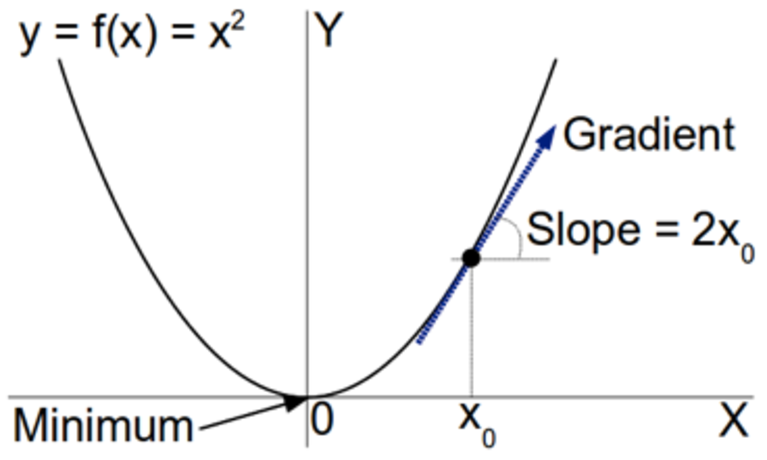
\includegraphics[width=3in]{FIGS/x_square}
\caption{The Archetypical Convex Function $f(x) = x^2$.}
\label{fig:xsquare}
\end{figure}

\begin{figure}
\centering
{\small
\begin{tabular}[t]{|l||l|}
\hline
Application & Objective \\
\hline
\hline
Least Squares & $\sum_{(u,y) \in \Omega} (x^Tu - y)^2$\\
Lasso~\cite{Tibshirani94regressionshrinkage} & $\sum_{(u,y) \in \Omega} (x^Tu - y)^2 + \mu  \|x\|_1$\\
Logisitic Regression & $\sum_{(u,y) \in \Omega} \log(1 + \exp( - y x^tu )$\\
Classification (SVM)& $\sum_{(u,y) \in \Omega} (1 - yx^{T}u)_{+}$\\
\hline
Recommendation & $\sum_{(i,j)\in\Omega} (L_i^T R_j - M_{ij})^2 + \mu\|L,R\|_F^2$\\
Labeling (CRF)~\cite{wallach:crf} & $\sum_{k} \left[ \sum_{j} x_j F_j(y_k, z_k) - \log Z(z_k) \right]$ \\
\hline
\end{tabular}}
\caption{Models currently Implemented in MADlib using the IGD-based
  approach\scriptsize In classification and regression methods, given
  a dataset $\Omega \subseteq \mathbb{R}^{N} \times \mathbb{R}$, we
  minimize the error of a predictor $x \in \mathbb{R}^N$ on a
  dataset. Given $(u,v) \in \Omega$, the methods above predict the
  value of $y$ by the equation $x^Tu$. One can add a regularization
  term to any regression or classification model, e.g., to combat
  overfitting. For example, in Lasso, we minimize the square loss
  against the data subject to an $\ell_1$ regularization.  In
  recommendation, given a matrix $M \in \mathbb{R}^{n \times m}$
  observed on a set of entries $\Omega \subseteq [n] \times [m]$, we
  fit a so called low-rank approximation, i.e., $L \in \mathbb{R}^{n
    \times k}$ and $R \in \mathbb{R}^{m \times k}$ for $k \ll
  \min\{m,n\}$ .  The low-rank matrix is regularized by the sums of the
  squares of its factors.  In Labeling with Conditional Random fields,
  we maximize the weights associated with features $(F_j)$ in the text
  predict the labels }
\label{fig:objs:grads}
\end{figure}

%% \paragraph*{Future Work and Challenges} We plan to work on three challenges: (1) improving performance, (2) an infrastructure to make tools in MADlib statistically robust, and (3) SAS-style Model Management. 
%% \begin{enumerate}
%% \item \textbf{Improving Performance}. IGDs are not a panacea. They
%%   have suboptimal runtime performance if extremely high precision is
%%   required. We plan to add in more both mathematical and systems-level
%%   optimization methods, which can be done transparently leveraging the
%%   decoupling provided by convex analysis.

%% \item \textbf{Increasing Robustness}. In its current version, MADlib
%%   encodes parameters of the algorithms (sometimes called
%%   hyperparameters) in the code itself. Some statistical techniques
%%   like regularization (a common technique to prevent overfitting or
%%   deal with poorly conditioned data) require that a user tune a
%%   parameter on their data. We would like to be able to expose such
%%   parameters in a generic way and then provide automated tuning
%%   techniques. In turn, our hope is to increase the robustness of these
%%   statistical tools automatically.

%% \item \textbf{Managing Models, SAS-style}. The term model management
%%   in the SAS literature is a distinct concept from the database
%%   term. The idea is to track how a model is derived, how robust its
%%   parameters are, which features are used in its construction. This
%%   has proved extremely useful in the SAS area to support higher-level
%%   business analytics. We plan to study this problem and develop an
%%   abstraction to support it.

%% \end{enumerate}

\subsection{Florida Contributions: Statistical Text Analytics}

%Importance of statistical text analysis 
The focus of the MADlib work at Florida has been to integrate statistical text analytics into a DBMS.
In many domains, structured
data and unstructured text are both important assets for data
analysis. The increasing use of text analysis in enterprise
applications has increased the expectation of customers and the
opportunities for processing big data. The state-of-the-art text
analysis tools are based on statistical models and
algorithms~\cite{}. With the goal to become a framework for
statistical methods for data analysis at scale, it is important for
MADlib to include basic statistical methods to implement text analysis
tasks.

% different text analysis tasks
Basic text analysis tasks include part-of-speech (POS) tagging,
named entity extraction (NER), and entity resolution (ER)~\cite{}.
Different statistical models and algorithms are implemented for each
of these tasks with different runtime-accuracy tradeoffs. For
example, an entity resolution task could be to find all mentions in
a text corpus that refer to a real-world entity $X$. Such a task can
be done efficiently by approximate string matching~\cite{}
techniques to find all mentions in text that approximately match the
name of entity $X$. However, such a method is not as accurate as the
state-of-the-art collective entity resolution algorithms based on
statistical models, such as Conditional Random Fields
(CRFs)~\cite{crftutorial}.

% our goal
% what we've done
\paragraph*{Pushing Statistical Text Analysis into MADlib}
Based on the MADlib framework, our group set out to implement
statistical methods in SQL to support various text analysis tasks.  We
use CRFs as the basic statistical model to perform more advanced text
analysis. Similar to Hidden Markov Models (HMM)~cite{}, CRFs are a
leading probabilistic model for solving many text analysis tasks,
including POS, NER and ER~\cite{needed}. To support sophisticated text
analysis, we implement four key methods: text feature extraction, most-likely inference
over a CRF (Viterbi), Markov-chain Monte Carlo inference, and
approximate string matching. 

\begin{table}
  \centering
\begin{tabular}{|c|c|c|c|}
  \hline
  % after \\: \hline or \cline{col1-col2} \cline{col3-col4} ...
  Statistical Methods & POS & NER & ER \\
  Text Feature Extraction & $\checkmark$ & $\checkmark$ & $\checkmark$ \\
  Viterbi Inference & $\checkmark$ & $\checkmark$ &  \\
  MCMC Inference &  & $\checkmark$ & $\checkmark$ \\
  Approximate String Matching &  &  & $\checkmark$ \\
  \hline
\end{tabular}
\caption{Statistical Text Analysis Methods}
\label{tab:uflmethods}
\end{table}

%% \dzw{Add query-driven text analysis? -- Motivation for query-driven
%% text analysis techniques for IE and ER. Compare to tasks that does
%% not need to be real-time query-driven (e.g., POS, feature
%% extraction).}

\textbf{Text Feature Extraction:} Text feature extraction is a step in
most statistical text analysis methods, and it can be an expensive
operation. To achieve high quality, CRF methods often assign hundreds
of features to each token in the document. Examples of such features
include: (1) dictionary features: {\it does this token exist in a
  provided dictionaries?}; (2) regex features: {\it does this token
  match a provided regular expressions?}; (3) edge features: {\it is
  the label of a token correlated with the label of a previous
  token?}; (4) word features: {\it does this the token appear in the
  training data?}; and (5) position features: {\it is this token is the
  first or last in the token sequence?}. The right combination of
features depends on the application, and so our supporting for feature
extraction heavily leverages the micro-programming interface provided
by MADlib.

\textbf{Approximate String Matching:} A recurring primitive operation
in text processing applications is the ability to match strings
approximately. The technique we use is based on qgrams~\cite{}. 
% This technique is an
% approximate string match that was first introduced in the SQouT
% project~\cite{}. 
We used the trigram module in PostgreSQL to create
and index 3-grams over text.  Given a string ``Tim Tebow'' we can
create a 3-gram by using a sliding window of 3 characters over this
text string. Given two strings we can compare the overlap of two sets
of corresponding 3-grams and compute a similarity as the approximate
matching score. This functionality comes packaged with PostgreSQL.

%The similarity between $term_1$ and $term_2$ is computed using the
%following equation:
%
%\begin{equation}\label{}
%    S(term_1, term_2) = \frac{|term_1 \cup
%    term_2|}{min\{|term_1|,|term_2|\}}.
%\end{equation}

Once we have the features, the next step is to perform inference on
the model. We also implemented two types of statitical inference
within the database: Viterbi (when we only want the most likely answer
from the model) and MCMC (when we want the probabilities or confidence
of an answer as well).

\textbf{Viterbi Inference:} The \textit{Viterbi} dynamic
programming algorithm~\cite{viterbi} is the popular algorithm to find
the top-k most likely labelings of a document for (linear chain) CRF
models. The following dynamic programming computes the top-1 label
sequence. (This can be easily extended to compute the top-k).

\vspace{-0.4cm}{\small
\begin{equation}\label{Equation:crf_viterbi}
V(i,y) = \left\{\begin{array}{lll}
    \max_{y'} (V(i-1,y') & &\\
    \quad + \sum^K_{k=1} \lambda_k f_k(y,y',x_i)), & $if$ & i\geq 0\\
    0, & $if$ & i = -1.
    \end{array}\right.
\end{equation}}

The Viterbi algorithm is recursive, so for macro-coordination we chose to implement it using a combination of recursive SQL and window aggregate functions.  A side-effect of our recursive SQL implementation is that it only runs over PostgreSQL versions 8.4 and later; it does not currently run in Greenplum.\jmh{Daisy, is the above correct?}

%% CHRIS: I AM NOT SURE THIS IS CORRECT!

\textbf{MCMC Inference:} Markov chain Monte Carlo (MCMC) methods are
classical sampling algorithms that can be used to estimate probability
distributions. We implemented two MCMC methods in MADlib: Gibbs
sampling and Metropolis-Hastings (MCMC-MH). The iterative Gibbs
sampling algorithm is shown in Figure~\ref{Algo:Gibbs}.

\begin{figure}
\hrulefill\\
{\small
\begin{algo}{Gibbs}{N}
    w_0 \: \CALL{Init}(); w \: w_0; |  // initialize|
    \FOR{idx = 1,...,N}
        i \: idx \% n; |  // propose variable to sample next|
        w' \sim \pi (w_{i}\mid w_{-i}) |  // generate sample|
        \RETURN{| | next | | w'} |  // return a new sample|
        w \: w'; |  // update current world|
    \ENDFOR
\end{algo}}
\hrulefill\\
\caption{Pseudo-code for MCMC Gibbs sampling algorithm over a model
with $n$ variables.}  \label{Algo:Gibbs}
\end{figure}
\jmh{Daisy, please complete discussion of macro-coordination style for this implementation.}

% main results, lessons, surprises
\paragraph*{Using the MADlib Framework} 
In our work we diverged from some of the macro-coordination lessons adopted by MADlib, and took advantage of features of PostgreSQL that are less portable.  These details will require refactoring to fit into the current MADlib design style,
In addition to the work reported above, there are a host of other features of both PostgreSQL and MADlib
that are valuable for text analytics: (1) text processing features such
as inverted indexes, trigram indexes for approximate string matching,
and array data types for model parameters, (2) powerful query processing
features such as recursive queries and window functions for passing
states between iterations, and (3) the existing modules in MADlib,
such as Naive Bayes and Sparse/Dense Matrix manipulations, are
building blocks to implement statistical text analysis
methods. Leveraging this diverse set of tools and techniques that are
already within the database allowed us to build a sophisticated text
analysis engine that has comparable raw performance to off-the-shelf
implementations, but runs natively in a DBMS close to the data~\cite{daisy1,daisy2}. 

%% Statistical methods can be implemented in a relational database
%% efficiently. Prior work~\cite{} shows comparable performance between
%% in-database SQL and off-the-shelf implementations. Real-time
%% query-driven text analysis can be supported using indexes over a large
%% document corpus, which can be orders-of-magnitude faster than an
%% off-line batch process.


%% \textbf{Query-Driven Techniques}

%% Information Extraction (Viterbi, Feature Extraction)

%% Entity Resolution (MCMC, Approximate String Matching)

%% \textbf{Future Work}

%% \begin{itemize}
%%   \item Performance Improvement (Feature Extraction)
%%   \item MPP Implementation
%%   \item POS/IE/ER models
%%   \item Text Analysis query interface design
%% \end{itemize}
%% Performance Improvement (Feature Extraction) MPP Implementation
%% POS/IE/ER models Query-driven Text Analysis Interface (including
%% key-word search and more advanced)

\section{Related Work: Ecosystem of Scalable Analytics}
\jmh{I think we need a pro-forma related work section that cites various efforts for scalable ML, particularly in open source.}
      Traditional analysts bring data to the code: see the SAS \textit{SEMMA}
      approach.  Import/export cycle with SAS, R, etc.  This will
      always exist, but it will be increasingly less useful.  There
      are active efforts to scale and parallelize these, but those are
      still quite limited, and companies like SAS are working hard to
      partner with approaches from below...

      The new model of scalable analytics depends on bringing the code
      to the data in a scalable storage/analysis framework.  So you
      can structure the space in terms of where the data lives.  Not
      going to get into \textit{what's better} here -- truth is that there
      are pros and cons, and many organizations use more than one.

      Things are really in flux.  Segments kinda like so:
      \begin{itemize}
          \item SQL universe has proprietary {\em data mining} toolkits, many of which date back to the 1990s.  These cost a lot and evolve very slowly.  Cite the Teradata research papers, IBM white book.  MADlib is an effort to raise all boats in this domain.
          \item HDFS/Hadoop universe is burgeoning.  Mahout is the center of energy for ML algorithms right now. (also System ML?)  Exciting trend there, and while the ML libraries are still quite young, they may evolve quickly.
          \item A variety of emerging in-memory distributed systems like Graphlab, Vowpal Wabbit, Spark, Pregel/Giraph.  These merit a close look.  Some of them present alternative architectures to traditional dataflow parallelism (e.g. GraphLab, VW).  Others are targeted to problems like graph algorithms that may prove to be weak spots for more general purpose systems (e.g. Graphlab, Pregel/Giraph).
        \end{itemize}



\section{MADlib Beta Release: Status Report and Future Direction}
\jmh{Do we need this?  or is the table and discussion up front enough?}
     Engineering team leading to Beta was XX Greenplum heads + 1
     Berkeley head.  Greenplum also donating ongoing automated
     testing on x OSes and y DBMS versions (PG \& GP, multiple
     versions of each).  Contributors from Wisconsin and Florida
     constitutes YYY heads to date.

     Expand the following from the user docs.  For each method, should be refs to literature on the algorithms being used.
     \begin{itemize}
         \item Stat and linear algebra fundamentals
         \item Descriptive statistics (deterministic, and one-pass approximation algorithms)
         \item Regression
         \item Unsupervised learning/Data mining
         \item Supervised learning
       \end{itemize}



\section{MADlib Futures}
\begin{itemize}
          \item Development of additional methods based on case studies in industry.  We welcome input on this front.
          \item Expand academic involvement.  Solicitation of experimental research methods from academia.  Currently lined up projects at U. Wisconsin and U. Florida (see if we can get Chris and Daisy testimonials for now; code soon.)  We welcome more collaboration with interested academics.
          \item Continued robustification of the codebase, with help from QA and engineering contributions at EMC/Greenplum on the PostgreSQL and Greenplum platforms.  We welcome offers of support from other teams to develop and maintain ports on other open-source and commercial platforms.
\end{itemize}
\section{Conclusion}



{\small \bibliographystyle{abbrv}
  \bibliography{chris.local.wopages} }

\end{document}
